\section{Stepper motors}
\label{sec:steppers}
This section gives a brief introduction into stepper motors and their control.
First, stepper motors and their types are described.
Then, a comparison of stepper driver ICs is given and some of the motion control technologies by Trinamic are described.

Stepper motors are a type of DC motors which move in discrete steps\cite{earl_all_nodate,carmine_fiore_stepper_2021}.
Such movement is achieved by their construction - they consist of a stator and a rotor, where the stator is made of coils
(two coils form a phase) wound on ridges, whereas the rotor consists is a ferromagnetic structure - either a permanent
magnet or a variable reluctance iron core\cite{carmine_fiore_stepper_2021}.

\subsection{Working principle}
\label{subsec:stepper_working_principle}
The basic working principle of stepper motors can be seen in the~Figure~\ref{fig:stepper_working_principle}.
In the Figure, we can see a three-phase bidirectional stepper motor.
First, the coils of the stator winding \textbf{A} are energized, which causes the ferromagnetic rotor to align with the magnetic field induced by the phase winding.
In the second step, the winding \textbf{B} is energized, causing the rotor magnetic field to realign with the newly induced magnetic field of the second winding.
This causes the motor to move.
In the next step, the winding \textbf{C} is energized, which again causes realignment of the rotor.
In the following steps, the coils are energized again but with different polarity making the rotor make a full turn.

\begin{figure}[H]
    \centering
    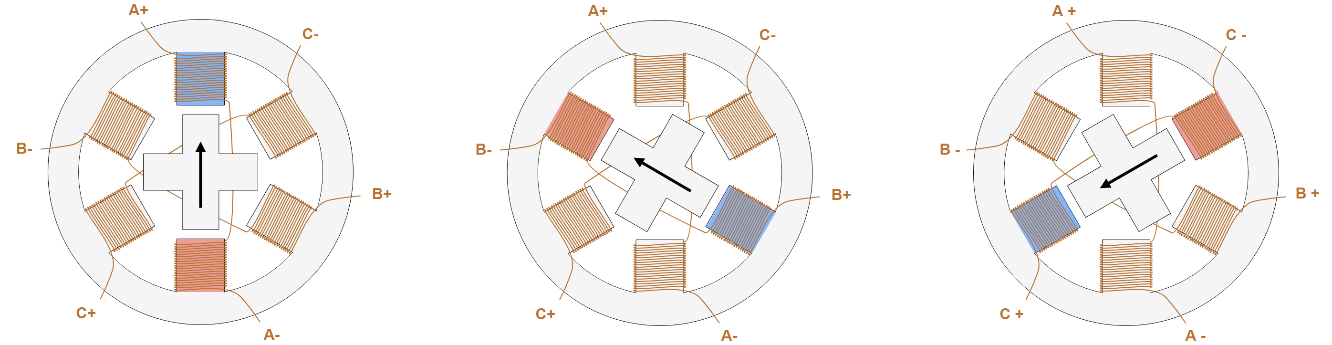
\includegraphics[width=\textwidth]{obrazky/stepper_principle}
    \caption{Working principle of a stepper motor~\cite{carmine_fiore_stepper_2021}.}
    \label{fig:stepper_working_principle}
\end{figure}

\subsection{Rotor}
\label{subsec:rotor}
There are three different constructions of rotors~\cite{carmine_fiore_stepper_2021}:
\begin{itemize}
    \item \textbf{Permanent magnet rotor} - utilizes a permanent magnet in the place of the stator.
    An advantage of this type of stator is good torque and also detent torque (the resistance of the motor shaft when no windings are energized)~\cite{carmine_fiore_stepper_2021}.
    \item \textbf{Variable reluctance rotor} - the rotor consists of a shaped iron core.
    The torques are generally lower and there is no detent torque~\cite{carmine_fiore_stepper_2021}.
    \item \textbf{Hybrid motor} - is created by combining a permanent magnet rotor with a variable reluctance rotor.
    There are two magnetic caps with teeths on top of each other that have an angular shift between them.
    The rotor is magnetized axially~\cite{carmine_fiore_stepper_2021}.
\end{itemize}

\subsection{Stator}
\label{subsec:stator}
The construction of stator depends on the number of phases the motor has.
Every phase consists of two windings and the windings can be center-tapped or not, which determines if the motor is bipolar or unipolar.
With unipolar windings, the center tapped lead is connected to the input voltage and the direction of the magnetic field is controlled by connecting ground to the other leads.
Bipolar motors do not have center tapped lead and the coil itself is controlled using a H-bridge.

\subsection{Phase Winding Energizing Techniques}
\label{subsec:winding_tech}
The way of energizing windings described in the Subsection~\ref{subsec:stepper_working_principle} is only one of four ways of controlling the windings.
This technique, where only one of the phases is energized at a time is called the wave mode.
it was described in detail in the Subsection~\ref{subsec:stepper_working_principle} and the sequence of energizing windings can be seen in the Figure~\ref{fig:stepper_wave_mode}.

\begin{figure}[H]
    \centering
    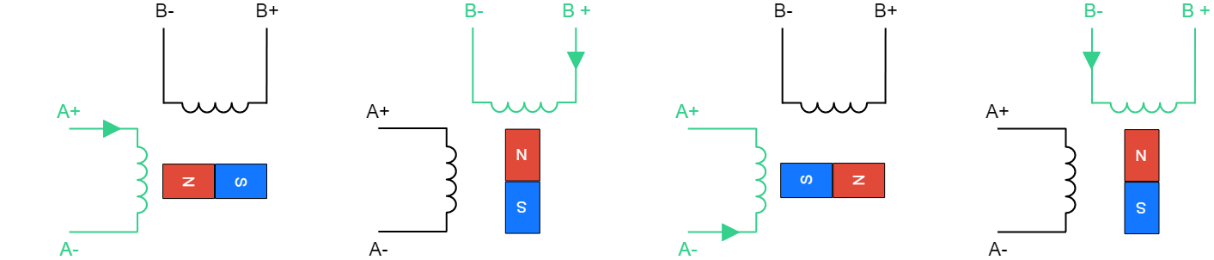
\includegraphics[width=\textwidth]{obrazky/wave_principle}
    \caption{Controlling stepper motor phase windings in wave mode~\cite{carmine_fiore_stepper_2021}.}
    \label{fig:stepper_wave_mode}
\end{figure}

\newpage
Another way of driving the motor is called the full-step mode.
In this mode, two phase windings are energized at the same time.
Changing the current direction in the winding causes the rotor to realign.
The advantage of this mode is higher torque as the magnetic field is stronger when the two of the phase windings are energized.
The working principle can be seen graphically in the Figure~\ref{fig:stepper_full_step_mode}.

\begin{figure}[H]
    \centering
    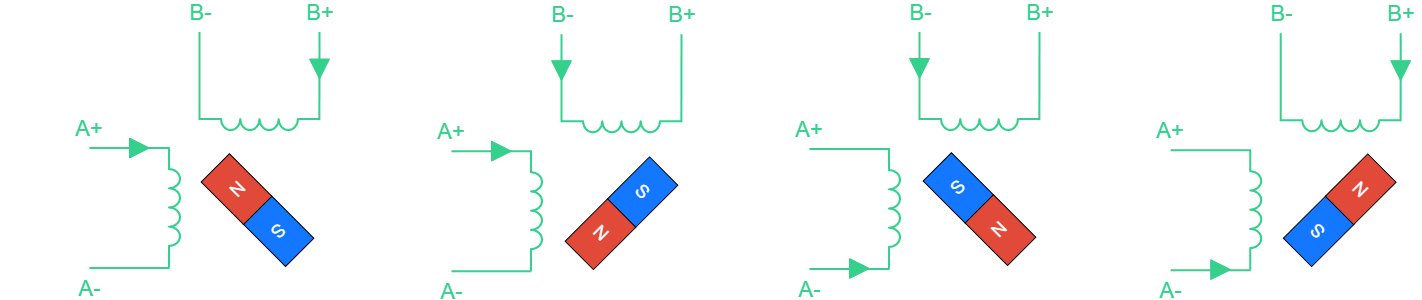
\includegraphics[width=\textwidth]{obrazky/full_step_principle}
    \caption{Controlling stepper motor phase windings in full step mode~\cite{carmine_fiore_stepper_2021}.}
    \label{fig:stepper_full_step_mode}
\end{figure}

Combining the wave mode and the full step mode results in a half-step mode.
In contrast to the previous driving modes, the step size of this mode is the half of the previous mode - in case of this virtual motor with permanent magnet motor 90\textdegree, therefore 45\textdegree.
This mode alternates between energizing only one phase winding and energizing both phase windings.
The disadvantage of this mode is that the produced torque is not constant as the torque is different when both phase windings are energized and when only one of them is.
The working principle can be seen in the Figure~\ref{fig:stepper_half_step_mode}.

\begin{figure}[H]
    \centering
    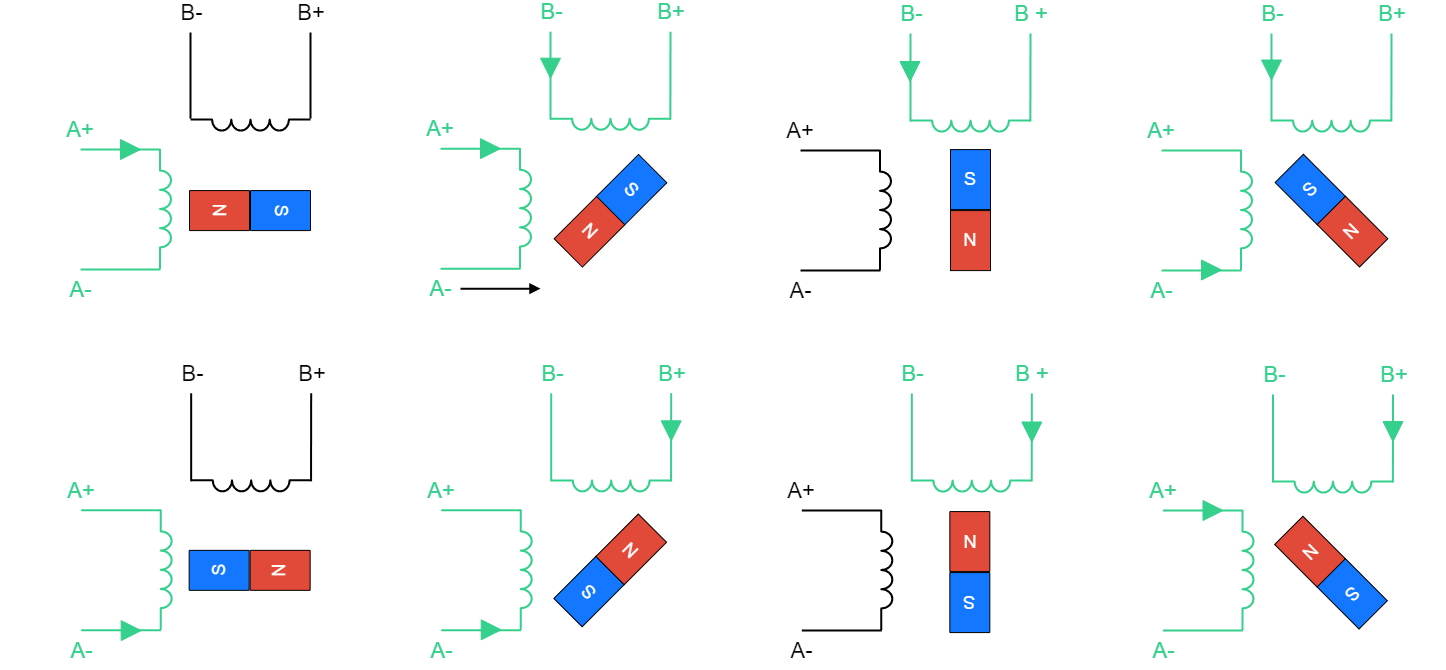
\includegraphics[width=\textwidth]{obrazky/half_step_principle}
    \caption{Controlling stepper motor phase windings in half step mode~\cite{carmine_fiore_stepper_2021}.}
    \label{fig:stepper_half_step_mode}
\end{figure}

The last technique for driving stepper motors is microstepping.
The advantage of this mode is that it reduces step size and has constant torque output~\cite{carmine_fiore_stepper_2021}.
The working principle for this mode is that the current flowing through the phase winding is controlled in some ratio, finely positioning the rotor as can be seen in the Figure~\ref{fig:microstepping}.
Microstepping is nowadays the prevalent way of stepper motor control as it allows for precision control and allows for constant torque.

\begin{figure}[H]
    \centering
    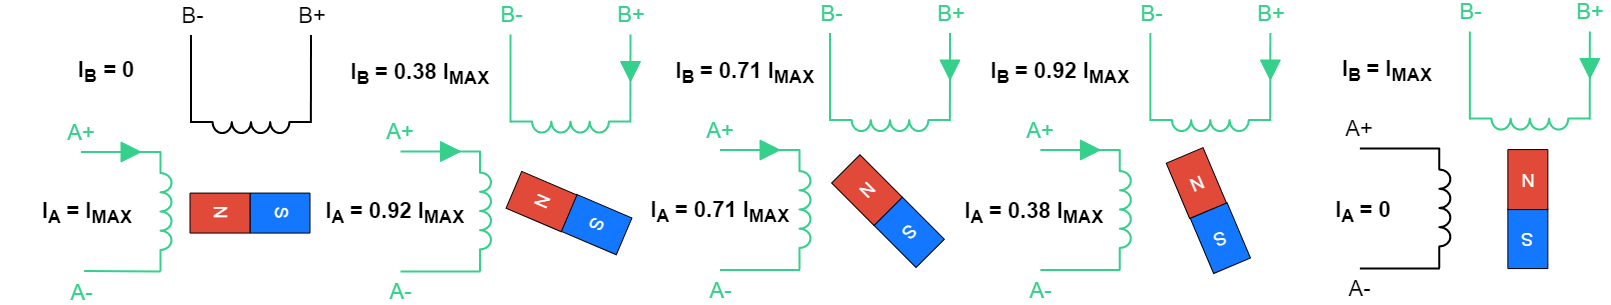
\includegraphics[width=\textwidth]{obrazky/microstepping}
    \caption{Controlling stepper motor phase windings in microstepping mode~\cite{carmine_fiore_stepper_2021}.}
    \label{fig:microstepping}
\end{figure}

\subsection{NEMA17 style stepper motor}
\label{subsec:nema}
In this Section, a typical NEMA17 style motor is described.
NEMA17 is a standard describes the flange size, where the number denotes the flange size in tenths of an inch\cite{reprap_nema_nodate}, in this case 1.7".
The NEMA 17 style motors are commonly used in 3D printers.
The specific motor is a 17HS4401, it is a two phase bipolar stepper motor with step angle of 1.8\textdegree s.
The motor's length is 40 mm, its rated current is 1.7~A, and it has a holding torque of 0.4~Nm\cite{noauthor_nema_nodate}.
An image of the motor can be seen in the Figure~\ref{fig:nema17}.

\begin{figure}[H]
    \centering
    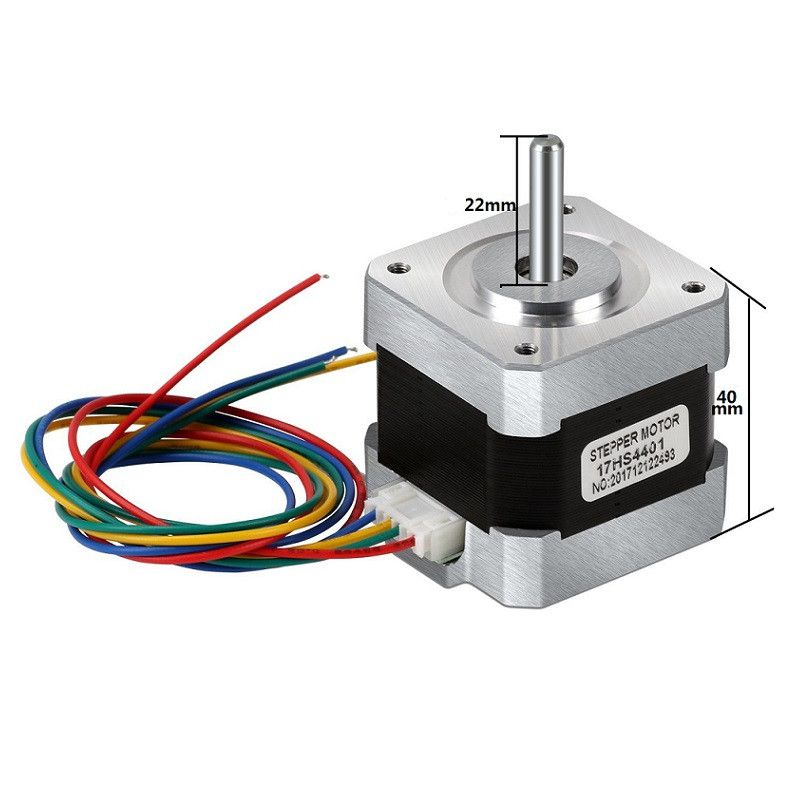
\includegraphics[width=0.5\textwidth]{obrazky/nema17}
    \caption{A typical look of a NEMA17 motor.}
    \label{fig:nema17}
\end{figure}

\subsection{Trinamic motion control technologies}
\label{subsec:trinamic_tech}
As we described in the Section~\ref{subsec:stepper_ic}, we decided to utilize Trinamic made driver \acs{ic}s and their stepper control technologies.
It is vital to describe these technologies as they have immediate impact on the driver performance and properties.

\subsubsection{MicroPlyer\texttrademark}
MicroPlyer\texttrademark is a microstepping interpolator.
The reason for the interpolator is that the drivers feature 256 microsteps per step and generating the stepping signal would be impractical if not impossible for some systems.
The driver is configured with the number of microsteps that the driver will consider a full step and the MicroPlyer\texttrademark interpolates the rest of the microsteps up to the 256 microsteps per step\cite{trinamic_microstepping_nodate}.

\subsubsection{Voltage Chopper Modes - SpreadCycle\texttrademark, StealthChop\texttrademark}
In order to define chopper modes, we first need to define the current control modes for a bipolar stepper motor.
The current control modes are the ON-phase, fast decay and slow decay.
These modes can be seen in the Figure~\ref{fig:current_phases}.

\begin{figure}[H]
    \centering
    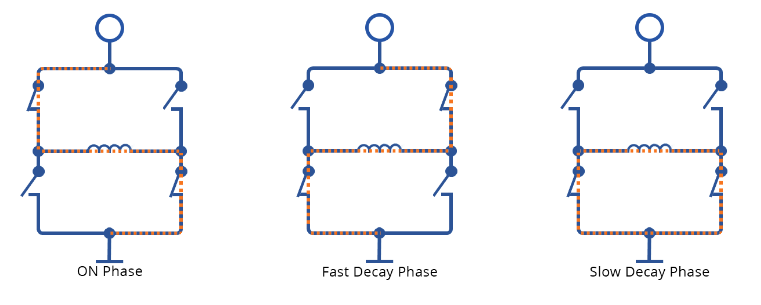
\includegraphics[width=\textwidth]{obrazky/winding_modes}
    \caption{Stepper motor winding control modes~\cite{trinamic_chopper_nodate}.}
    \label{fig:current_phases}
\end{figure}

The current in the winding is controlled using voltage choppers.
First, a very high voltage is applied to the winding, which causes current rise in the winding, when the current exceeds specific limit, the voltage is chopped (turned off).
When the current drops below a specified limit, the very high voltage is turned back on.
Using this approach, it is possible to maintain a relatively constant current in the winding\cite{trinamic_chopper_nodate}.

When using a Constant T\_OFF Current Chopper, the basic chopper principle is enhanced by first, energizing the winding, then utilizing fast-decay and then slow decay.
This is a commonly used chopper mode as it is quite simple, but it causes motor vibration, and the high pitch noise.
This problem is caused by the relationship between the fast decay and slow decay phase, resulting in the average current being lower than the desired target.
This means that there are moments when the motor has no torque, which in turn causes vibrations\cite{trinamic_chopper_nodate}.
The graph showing the winding current in time can be seen in the Figure~\ref{fig:t_off_chopper}.

\begin{figure}[H]
    \centering
    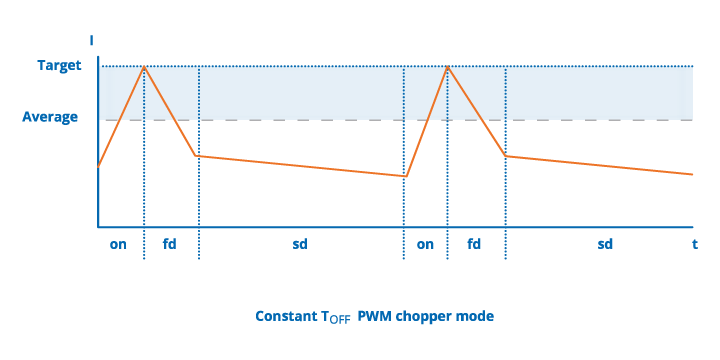
\includegraphics[width=\textwidth]{obrazky/t_off_chopper}
    \caption{Constant T\_OFF Chopper Mode~\cite{trinamic_chopper_nodate}.}
    \label{fig:t_off_chopper}
\end{figure}

The SpreadCycle\texttrademark current chopper is an improvement over the Constant T\_OFF Current chopper.
According to Trinamic, it automatically applies a fitting relation between slow decay and fast decay to create the optimal fast decay for that cycle\cite{trinamic_chopper_nodate}.
This technique leads to the average current matching the target current and the current wave resembles sine wave.
This technology also remains effective at higher RPMs, where the classic constant T\_OFF Chopper shows current deformations\cite{trinamic_chopper_nodate}.
The current in time can be seen in the Figure~\ref{fig:spread_cycle}.

\begin{figure}[H]
    \centering
    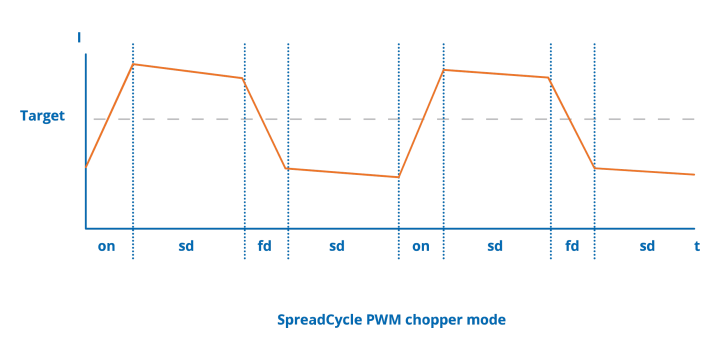
\includegraphics[width=\textwidth]{obrazky/spread_cycle}
    \caption{The SpreadCycle\texttrademark Mode current graph~\cite{trinamic_chopper_nodate}.}
    \label{fig:spread_cycle}
\end{figure}

StealthChop\texttrademark is the most advanced voltage chopper technology Trinamic drivers provide.
The chopper completely silences stepper motors by eliminating the noise cause by unsynchronized motor coil chopper operation, PWM jitter and regulation noise at the sense resistors\cite{trinamic_chopper_nodate}.
The chopper modulates the current using the PWM duty cycle, which minimizes the current ripple\cite{trinamic_chopper_nodate}.
Adjusting the PWM duty cycle also results in a perfect current sine wave and minimizing the current ripple minimizes Eddy currents in the stator, which in turn leads to less power loss and increase efficiency\cite{trinamic_chopper_nodate}.


\subsubsection{StallGuard\texttrademark}
The StallGuard\texttrademark technology utilizes the back EMF (ElectroMotive Force) to analyze the load of the motor.
This provides the drivers with a sensorless load measurement.
This technology may be utilized for sensorless homing, self-calibration or distance measurement.
The StallGuard\texttrademark technology also prevents step loss when the axis is obstructed\cite{trinamic_trinamic_nodate}.

\subsubsection{CoolStep\texttrademark}
CoolStep\texttrademark is a technology that adjusts the motor current based on the feedback provided by the StallGuard\texttrademark technology.
This technology always drives the motor at the minimum required current sufficient for driving the actual load.
That leads to reduced current consumption and also reduces heat generation.
The technology also allows for temporary current boosts.
An example of the dependency on the motor current on the load torque can be seen in the Figure~\ref{fig:torque_current}.

\begin{figure}[H]
    \centering
    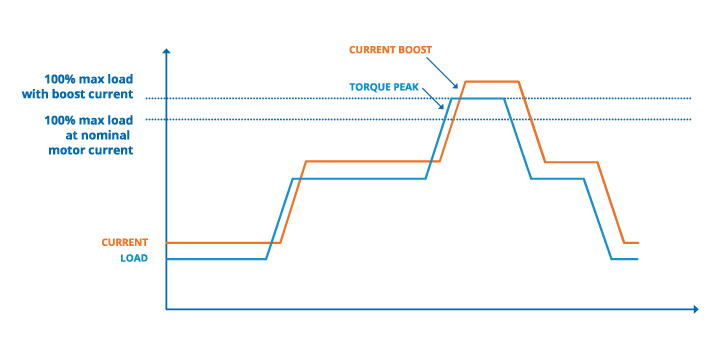
\includegraphics[width=\textwidth]{obrazky/Trinamic_CoolStep}
    \caption{The Trinamic CoolStep\texttrademark technology~\cite{trinamic_trinamic_nodate}.}
    \label{fig:torque_current}
\end{figure}
